\documentclass[a4paper]{article}

% Packages
\usepackage{amsmath}
\usepackage{amssymb}
\usepackage{amsthm}
\usepackage{bold-extra}
\usepackage{fancyhdr}
\usepackage{geometry}
\usepackage{graphicx}
\usepackage{hyperref}
\usepackage{ifthen}
\usepackage[utf8]{inputenc}
\usepackage{multirow}
\usepackage{needspace}
\usepackage{parskip}
\usepackage{stmaryrd}
\usepackage{listings}
\usepackage[T1]{fontenc}
\usepackage{longtable}
\usepackage{comment}
\usepackage{enumerate}
\usepackage{xspace}
\usepackage{textcomp}
\usepackage{array}

\usepackage{tikz}
\usetikzlibrary{automata,positioning,shapes.geometric}
\usepackage{tikzsymbols}
\usepackage{todonotes}

\lstset{language=Java, numbers=left, showstringspaces=false, tabsize=4}
\geometry{a4paper, left=25mm,right=25mm, top=25mm, bottom=25mm}

% check for the existence of commands
\newcommand{\checkfor}[3]{%
  \ifcsname#1\endcsname%
  #2
  \else%
  #3
  \fi%
}

\checkfor{exnumber}{}{\newcommand{\exnumber}{-1}}

\newcommand{\exercisepagebreak}{\checkfor{isexercise}{\pagebreak}{}}
\newcommand{\solutionpagebreak}{\checkfor{isexercise}{}{\pagebreak}}

\setcounter{section}{\exnumber{}}

\numberwithin{equation}{section}
\numberwithin{figure}{section}
\numberwithin{table}{section}
\renewcommand{\qedsymbol}{\textsc{q.e.d.}}
\renewenvironment{proof}[1][\proofname]{{\bfseries #1: }}{\qed}
\newtheoremstyle{defstyle}{10pt}{5pt}{\addtolength{\leftskip}{2\leftmargini}\addtolength{\rightskip}{2\leftmargini}}{-1\leftmargini}{\scshape\bfseries}{:}{\newline}{#1 #2\ifthenelse {\equal {#3}{}} {}{ (\text{\textsc{#3}})}}{}
\newtheoremstyle{thmstyle}{10pt}{5pt}{\addtolength{\leftskip}{2\leftmargini}\addtolength{\rightskip}{2\leftmargini} \slshape}{-1\leftmargini}{\scshape\bfseries}{:}{\newline}{#1 #2\ifthenelse {\equal {#3}{}} {}{ (\text{\textsc{#3}})}}{}
\newtheoremstyle{exstyle}{10pt}{5pt}{\addtolength{\leftskip}{2\leftmargini}\addtolength{\rightskip}{2\leftmargini}}{-1\leftmargini}{\scshape\bfseries}{:}{\newline}{#1 #2\ifthenelse {\equal {#3}{}} {}{ (\text{\textsc{#3}})}}{}
\newtheoremstyle{algostyle}{10pt}{5pt}{\addtolength{\leftskip}{2\leftmargini}\addtolength{\rightskip}{2\leftmargini}}{-1\leftmargini}{\scshape\bfseries}{:}{\newline}{#1\ifthenelse {\equal {#3}{}} { #2}{ \text{\textsc{#3}}}}{}
\theoremstyle{defstyle}
\newtheorem{mydef}{Definition}[section]
\theoremstyle{thmstyle}
\newtheorem{mythm}{Theorem}[section]
\newtheorem{mylem}[mythm]{Lemma}
\newtheorem{myprop}[mythm]{Proposition}
\theoremstyle{exstyle}
\newtheorem{myex}{Example}[section]
\theoremstyle{algostyle}
\newtheorem{myalgo}{Algorithm}

% Define programming and solution environment and only use if enabled
\checkfor{isprog}{
  % Define exercise environment
  \newcounter{exercise}
  \newenvironment{exercise}[1]{\refstepcounter{exercise}\label{ex\theexercise}\section*{Programming Exercise \theexercise \hfill (#1 Points)}}{}
  \checkfor{isexercise}{
    % Programming exercise
    \excludecomment{solution}
    \excludecomment{onlysolution}
    \newenvironment{onlyexercise}{}{}
    \newcommand{\extitle}{Programming Exercise}
  }{
    % Programming solution
    \newenvironment{solution}{\label{sol\theexercise}\subsection*{Solution: \hrulefill}}{}
    \newenvironment{onlysolution}{}{}
    \excludecomment{onlyexercise}
    \newcommand{\extitle}{Programming Solution}
    }
}{
  % Define exercise environment
  \newcounter{exercise}
  \newenvironment{exercise}[1]{\refstepcounter{exercise}\label{ex\theexercise}\section*{Exercise \theexercise \hfill (#1 Points)}}{}
  \checkfor{isexercise}{
    % Theoretical exercise
    \excludecomment{solution}
    \excludecomment{onlysolution}
    \newenvironment{onlyexercise}{}{}
    \newcommand{\extitle}{Exercise Sheet}
  }{
    % Theoretical solution
    \newenvironment{solution}{\label{sol\theexercise}\subsection*{Solution: \hrulefill}}{}
    \newenvironment{onlysolution}{}{}
    \excludecomment{onlyexercise}
    \newcommand{\extitle}{Solution}
  }
}

% Define header
\pagestyle{fancy}
\fancyhf{} % Clear all headers
\setlength{\headsep}{25pt}
\cfoot{\thepage} % Page numbers
\lhead{ % Header-Definition
  % Logo
  \begin{tabular}[b]{l l}
      \multirow{2}{38mm}{
        \raisebox{-3.6mm}[0pt][0pt]{
          
\includegraphics[height=14mm]{../i2}
        }
      }
      & Lehrstuhl f{\"u}r Informatik 2 \\
      & Software Modeling and Verification
    \end{tabular}
}
\rhead{ % Header-Definition
  % Course name
  \begin{tabular}[b]{r}
    Compiler Construction 2025\\
    \extitle{} \exnumber
  \end{tabular}
}
\AtBeginDocument{
  \vspace*{-30pt}
  apl.\ Prof.\ Dr.\ Thomas Noll\hfill Daniel Zilken, Roy Hermanns
  \vspace{5mm}
}


\newcommand{\header}[1]{
  % Header
  \begin{center}
    {\huge \textbf{Compiler Construction 2025}}\\
    \vspace*{1\baselineskip}%
    {\huge \textbf{--- \extitle{} \exnumber{} ---}}\\
    \checkfor{isexercise}{
      \vspace*{1\baselineskip}
      \checkfor{isprog}{
        %Upload in Moodle until #1 before the exercise class.
      }{
        Upload in Moodle or hand in until #1 before the exercise class.
      }
    }{}
    \vspace*{1.5\baselineskip}
    \hrule
  \end{center}
}

% Change numbering to (a) and (i)
\renewcommand{\labelenumi}{(\alph{enumi})}
\renewcommand{\labelenumii}{(\roman{enumii})}

% Custom commands
\newcommand{\TODO}[1]{\color{red}\textbf{TODO:} #1\color{black}}

% Macros
\newcommand{\set}[1]{\ensuremath{\left\{ #1 \right\}}}
\newcommand{\Nats}{\ensuremath{\mathbb{N}}}
\newcommand{\Reals}{\ensuremath{\mathbb{R}}}

\newcommand{\PTIME}{\mbox{\rm PTIME}}
\newcommand{\PSPACE}{\mbox{\rm PSPACE}}
\newcommand{\coNP}{\mbox{\rm coNP}}
\newcommand{\NP}{\mbox{\rm NP}}
\newcommand{\poly}{\mbox{\rm poly}}
\newcommand{\coPTIME}{\mbox{\rm coPTIME}}
\newcommand{\coPSPACE}{\mbox{\rm coPSPACE}}
\newcommand{\NPSPACE}{\mbox{\rm NPSPACE}}
\def\EXPTIME{\text{\rm EXPTIME}}
\def\doubleEXPTIME{\text{\rm 2EXPTIME}}

% Lecture specific commands
\renewcommand{\L}{{\cal L}}
\newcommand{\numberone}{\ensuremath{\set{1, \dots, 9}}}
\newcommand{\numberzero}{\ensuremath{\set{0, \dots, 9}}}
\newcommand{\eps}{\ensuremath{\varepsilon}}
\newcommand{\sem}[1]{\llbracket#1\rrbracket}
\newcommand{\la}{\ensuremath{\textsf{la}}}
\newcommand{\fir}{\ensuremath{\textsf{fi}}}
\newcommand{\first}{\ensuremath{\textsf{first}}}
\newcommand{\fo}{\ensuremath{\textsf{fo}}}
\newcommand{\follow}{\ensuremath{\textsf{follow}}}
\newcommand{\cyl}[1]{\ensuremath{\mathit{Cyl}(#1)}}
\newcommand{\icompiler}[0]{\texttt{i2Compiler}}
\newcommand{\while}[0]{\textit{WHILE}\xspace}


\usepackage{mdwlist}
\usepackage{algorithm2e}
\usepackage{mathtools}
\usepackage{csquotes}

\begin{document}

\header{November 23nd}

\begin{onlysolution}
  \begin{center}
    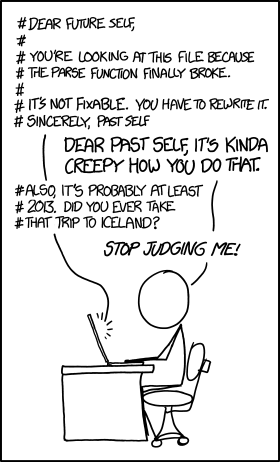
\includegraphics[scale=0.5]{xkcd_future_self}

    \scriptsize Credit: \href{https://xkcd.com/1421/}{https://xkcd.com/1421/}
  \end{center}
\end{onlysolution}

\section*{General Remarks}
\begin{itemize}
  %
\item If you have questions regarding the exercises, feel free to write us an email:
\[\text{   \href{mailto:cc22@i2.informatik.rwth-aachen.de}{cc22@i2.informatik.rwth-aachen.de}}
\]
%
%
\item Exercises are \emph{optional}, i.e., not required for admission to exams. However, corrections to students’ solutions are provided as annotations to the submissions.
%
\item You can hand in your solution to the tasks digitally in the Moodle room. Alternatively, you can hand in your solution to the tasks at our chair in the corresponding box or before the exercise class.
%
\item Please hand in your solutions in \emph{groups of four} and hand in only one solution per group. You can use the forum in this Moodle room to find group members.
\end{itemize}

%
% Source code
%
% \newcommand{\code}[1]{\ensuremath{\mathbf{\mathsf{#1}}}}
% \newcommand{\code}[1]{\text{\texttt{#1}}}
\newcommand{\code}[1]{{\bl{\text{\texttt{{\upshape#1}}}}}}
\newcommand{\Code}[1]{{\alert{\text{\texttt{{\upshape#1}}}}}}
\newcommand{\lbl}[2]{[#2]^{#1}}
\newcommand{\DO}{\code{do}}
\newcommand{\ELSE}{\code{else}}
\newcommand{\END}{\code{end}}
% \newcommand{\FOR}{\code{for}}
\newcommand{\IF}{\code{if}}
\newcommand{\ITE}[3]{\IF~#1~\THEN~#2~\ELSE~#3~\END}
% \newcommand{\NIL}{\code{nil}}
\newcommand{\THEN}{\code{then}}
% \newcommand{\TO}{\code{to}}
\newcommand{\WD}[2]{\WHILE~#1~\DO~#2~\END}
\newcommand{\WHILE}{\code{while}}
%
% Sets
%
\newcommand{\AExp}{\set{AExp}}
\newcommand{\AvExp}{\set{AE}}
\newcommand{\AG}{\set{AG}}
\newcommand{\AI}{\set{AI}}
\newcommand{\AM}{\set{AM}}
\newcommand{\Att}{\set{Att}}
\newcommand{\BExp}{\set{BExp}}
\newcommand{\bigO}[1]{\mathcal{O}(#1)}
\newcommand{\Blk}{\set{Blk}}
\newcommand{\Block}{\set{Blk}}
\newcommand{\Bool}{\mathbb{B}}
\newcommand{\Char}{\Omega}
\newcommand{\CFG}[1]{\set{CFG}_{#1}}
\newcommand{\CFL}[1]{\set{CFL}_{#1}}
\newcommand{\Cmd}{\set{Cmd}}
\newcommand{\Con}{\set{Con}}
\newcommand{\Dcl}{\set{Dcl}}
\newcommand{\Dep}{\set{D}}
% \newcommand{\DEP}{\mathfrak{D}}
\newcommand{\DFA}[1]{\set{DFA}_{#1}}
\newcommand{\DS}{\set{DS}}
\newcommand{\Env}{\set{Env}}
\newcommand{\Equ}{\set{E}}
\newcommand{\EVar}{\set{Ext}}
\newcommand{\Exp}{\set{Exp}}
\newcommand{\FP}{\set{FP}}
\newcommand{\Ide}{\set{Ide}}
\newcommand{\Inh}{\set{Inh}}
\newcommand{\Int}{\mathbb{Z}}
\newcommand{\IR}{\set{IR}}
\newcommand{\is}{\set{is}}
\newcommand{\IS}{\set{IS}}
\newcommand{\IVar}{\set{Int}}
\newcommand{\Lab}{\set{Lab}}
\newcommand{\LAG}{\set{LAG}}
%\newcommand{\LALR}[1]{\set{LALR}(#1)}
\newcommand{\Lev}{\set{Lev}}
\newcommand{\LL}[1]{\set{LL}(#1)}
\newcommand{\Loc}{\set{Loc}}
\newcommand{\LR}[1]{\set{LR}(#1)}
\newcommand{\LV}{\set{LV}}
\newcommand{\MS}{\set{MS}}
\newcommand{\Nat}{\mathbb{N}}
\newcommand{\NFA}[1]{\set{NFA}_{#1}}
\newcommand{\Off}{\set{Off}}
%\newcommand{\OVar}{\set{Out}}
\newcommand{\PC}{\set{PC}}
\newcommand{\Pgm}{\set{Pgm}}
\newcommand{\PS}{\set{PS}}
\newcommand{\Rat}{\mathbb{Q}}
\newcommand{\RE}[1]{\set{RE}_{#1}}
\newcommand{\Real}{\mathbb{R}}
\newcommand{\RS}{\set{RS}}
%\newcommand{\set}[1]{\ensuremath{\mathit{#1}}}
%\newcommand{\set}[1]{\mathit{#1}}
\newcommand{\Size}{\set{Size}}
%\newcommand{\SLR}[1]{\set{SLR}(#1)}
\newcommand{\SP}{\set{SP}}
\newcommand{\Stt}{\set{Stt}}
\newcommand{\Syn}{\set{Syn}}
\newcommand{\Tab}{\set{Tab}}
\newcommand{\Trn}{\set{Trn}}
\newcommand{\Type}{\set{Type}}
\newcommand{\Val}{\set{V}}
\newcommand{\VAL}{\set{Val}}
\newcommand{\Var}{\set{Var}}
%
% Mappings
%
\newcommand{\act}[1]{%
  \def\temp{#1}%
  \map{act}\ifx\empty\temp\else(#1)\fi%
}
% \newcommand{\aexpsem}[1]{%
%   \def\temp{#1}%
%   \mathfrak{A}\ifx\empty\temp\else\semantics{#1}\fi%
% }
\newcommand{\amsem}[1]{%
  \def\temp{#1}%
  \ifx\empty\temp\else\semantics{#1}\fi%
}
\newcommand{\atrans}[1]{%
  \def\temp{#1}%
  \map{at}\ifx\empty\temp\else(#1)\fi%
}
\newcommand{\att}[1]{%
  \def\temp{#1}%
  \map{att}\ifx\empty\temp\else(#1)\fi%
}
\newcommand{\base}[1]{%
  \def\temp{#1}%
  \map{base}\ifx\empty\temp\else(#1)\fi%
}
% \newcommand{\bexpsem}[1]{%
%   \def\temp{#1}%
%   \mathfrak{B}\ifx\empty\temp\else\semantics{#1}\fi%
% }
% \newcommand{\blocksem}[1]{%
%   \def\temp{#1}%
%   \mathfrak{K}\ifx\empty\temp\else\semantics{#1}\fi%
% }
\newcommand{\btrans}[1]{%
  \def\temp{#1}%
  \map{bt}\ifx\empty\temp\else(#1)\fi%
}
% \newcommand{\cmdsem}[1]{%
%   \def\temp{#1}%
%   \mathfrak{C}\ifx\empty\temp\else\semantics{#1}\fi%
% }
\newcommand{\ctrans}[1]{%
  \def\temp{#1}%
  \map{ct}\ifx\empty\temp\else(#1)\fi%
}
\newcommand{\DBA}[1]{\map{DBA}(#1)}
%\newcommand{\dclsem}[1]{%
%  \def\temp{#1}%
%  \mathfrak{D}\ifx\empty\temp\else\semantics{#1}\fi%
%}
\newcommand{\dom}[1]{\map{dom}(#1)}
\newcommand{\DTA}[1]{\map{DTA}(#1)}
\newcommand{\dtrans}[1]{%
  \def\temp{#1}%
  \map{dt}\ifx\empty\temp\else(#1)\fi%
}
\newcommand{\etrans}[1]{%
  \def\temp{#1}%
  \map{et}\ifx\empty\temp\else(#1)\fi%
}
\newcommand{\Eval}[1]{%
  \def\temp{#1}%
  \map{eval}\ifx\empty\temp\else(#1)\fi%
}
\newcommand{\final}{\map{final}}
%\newcommand{\first}[2]{%
%  \def\temp{#2}%
%  \map{first}_{#1}\ifx\empty\temp\else(#2)\fi%
%}
%\newcommand{\fir}[1]{%
%  \def\temp{#1}%
%  \map{fi}\ifx\empty\temp\else(#1)\fi%
%}
%\newcommand{\flow}{\map{flow}}
%\newcommand{\follow}[2]{%
%  \def\temp{#2}%
%  \map{follow}_{#1}\ifx\empty\temp\else(#2)\fi%
%}
%\newcommand{\fol}[1]{%
%  \def\temp{#1}%
%  \map{fo}\ifx\empty\temp\else(#1)\fi%
%}
\newcommand{\FV}{\map{Var}}
\newcommand{\gen}{\map{gen}}
\newcommand{\goto}[1]{%
  \def\temp{#1}%
  \map{goto}\ifx\empty\temp\else(#1)\fi%
}
\newcommand{\inh}[1]{%
  \def\temp{#1}%
  \map{inh}\ifx\empty\temp\else(#1)\fi%
}
\newcommand{\ic}[1]{%
  \def\temp{#1}%
  \map{trans}\ifx\empty\temp\else(#1)\fi%
}
\newcommand{\init}{\map{init}}
\newcommand{\ktrans}[1]{%
  \def\temp{#1}%
  \map{kt}\ifx\empty\temp\else(#1)\fi%
}
\newcommand{\kil}{\map{kill}}
%\newcommand{\la}[1]{%
%  \def\temp{#1}%
%  \map{la}\ifx\empty\temp\else(#1)\fi%
%}
\newcommand{\lr}[1]{%
  \def\temp{#1}%
  \map{lr_0}\ifx\empty\temp\else(#1)\fi%
}
\newcommand{\map}[1]{\ensuremath{\mathrm{#1}}}
\newcommand{\mc}[1]{%
  \def\temp{#1}%
  \map{code}\ifx\empty\temp\else(#1)\fi%
}
\newcommand{\pgmsem}[1]{%
  \def\temp{#1}%
%  \mathfrak{M}\ifx\empty\temp\else\semantics{#1}\fi%
  \ifx\empty\temp\else\semantics{#1}\fi%
}
\newcommand{\sbtrans}[1]{%
  \def\temp{#1}%
  \map{sbt}\ifx\empty\temp\else(#1)\fi%
}
\newcommand{\sctrans}[1]{%
  \def\temp{#1}%
  \map{sct}\ifx\empty\temp\else(#1)\fi%
}
\newcommand{\size}[1]{%
  \def\temp{#1}%
  \map{size}\ifx\empty\temp\else(#1)\fi%
}
%\newcommand{\st}{\map{st}}
\newcommand{\st}{\sym{st}}
\newcommand{\syn}[1]{%
  \def\temp{#1}%
  \map{syn}\ifx\empty\temp\else(#1)\fi%
}
\newcommand{\sync}[1]{%
  \def\temp{#1}%
  \map{sync}\ifx\empty\temp\else(#1)\fi%
}
\newcommand{\update}[1]{%
  \def\temp{#1}%
  \map{update}\ifx\empty\temp\else(#1)\fi%
}
\newcommand{\val}[1]{%
  \def\temp{#1}%
  v\ifx\empty\temp\else(#1)\fi%
}
\newcommand{\vtrans}[1]{%
  \def\temp{#1}%
  \map{vt}\ifx\empty\temp\else(#1)\fi%
}
\newcommand{\vtype}[1]{%
  \def\temp{#1}%
  \map{vtype}\ifx\empty\temp\else(#1)\fi%
}
%
% Automata and grammars
%
\newenvironment{automaton}[1]{
  \begin{tikzpicture}[->,>=triangle 45,shorten >=1pt,auto,node distance={#1},thick,bend angle=20,double distance=2pt]
  \tikzstyle{every state}=[draw,ellipse,inner sep=3pt,minimum size=10mm]
  \tikzstyle{initial}=[initial by arrow,initial text={}]
}{
  \end{tikzpicture}
}
\newenvironment{depgraph}{
  \begin{tikzpicture}[auto,inner sep=1pt,color=rwth,
    level distance=25mm,sibling distance=50mm,node distance=10mm]
    \tikzstyle{every node}=[draw=none]
    \tikzstyle{edge from parent}=[-,draw,thick]
}{
  \end{tikzpicture}
}
\newenvironment{syntaxtree}{
  \begin{tikzpicture}[level distance=12mm,sibling distance=10mm,inner sep=2pt,color=rwth,anchor=base]
%  \tikzstyle{every node}=[draw=none,text depth=2pt]
  \tikzstyle{every node}=[draw=none]
  \tikzstyle{edge from parent}=[-,draw,thick]
}{
  \end{tikzpicture}
}
\newcommand{\accept}{\token{accept}}
\newcommand{\ag}{\mathfrak{A}}
\newcommand{\auto}{\mathfrak{A}}
\newcommand{\below}[1]{\stackrel{#1}{\hookrightarrow}}
\newcommand{\bt}{\mathfrak{B}}
\newcommand{\dep}{\to}
\newcommand{\dertree}[2]{
  \begin{syntaxtree}
    \node [label={[black]right:#1}] {$\nt{Asg}$}
	    child { node [label={[black]left:#2}] {$\nt{Var}$} }
	    child { node [label={[black]right:#2}] {$\nt{Exp}$}
	      child { node [label={[black]right:#2}] {$\nt{Sum}$}
	        child { node [label={[black]left:#2}] {$\nt{Var}$} }
	        child { node [label={[black]right:#2}] {$\nt{Con}$} } } };
	\end{syntaxtree}
}
\newcommand{\error}{\token{error}}
\newcommand{\ilTo}[1]{\stackrel{#1}{\To}_l}
\newcommand{\irTo}[1]{\stackrel{#1}{\To}_r}
\newcommand{\lTo}{\To_l}
\newcommand{\NBA}[1]{\set{NBA}(#1)}
\newcommand{\NTA}[1]{\set{NTA}(#1)}
\newcommand{\nt}[1]{\ensuremath{\mathit{#1}}}
\newcommand{\pop}{\token{pop}}
\newcommand{\reduce}[1]{\token{red}\,#1}
\newcommand{\rTo}{\To_r}
\newcommand{\shift}{\token{shift}}
\newcommand{\To}{\Rightarrow}
%\newcommand{\token}[1]{{\color{blue}\text{\textsf{#1}}}}
\newcommand{\token}[1]{\ensuremath{\mathsf{#1}}}
\newcommand{\trans}{\vdash}
%
% Miscellaneous
%
\newcommand{\AND}{\wedge}
\newcommand{\angles}[1]{\langle#1\rangle}
\newcommand{\antlr}{\texttt{ANTLR}\xspace}
%\newcommand{\ao}[1]{\fbox{\sym{\color{black}#1}}}
\newcommand{\ao}[1]{\fbox{\sym{#1}}}
\newcommand{\bison}{\texttt{bison}\xspace}
\newcommand{\bl}[1]{{\color{rwth}#1}}
\newcommand{\blank}{\char32}
\newcommand{\ca}{\sym{ca}}
\newcommand{\contradiction}{\lightning}
\newcommand{\df}{:=}
\newcommand{\dif}{\sym{dif}}
\newcommand{\displayskips}{
  \addtolength{\abovedisplayshortskip}{-0.75ex}
  \addtolength{\abovedisplayskip}{-0.75ex}
  \addtolength{\belowdisplayshortskip}{-0.75ex}
  \addtolength{\belowdisplayskip}{-0.75ex}
%  \setlength{\abovedisplayshortskip}{1ex}
%  \setlength{\abovedisplayskip}{1ex}
%  \setlength{\belowdisplayshortskip}{1ex}
%  \setlength{\belowdisplayskip}{1ex}
}
\newcommand{\dlink}{\sym{dl}}
%\newcommand{\eps}{\varepsilon}
\newcommand{\evf}[2]{\langle#1,\!#2\rangle}
\newcommand{\FALSE}{\mathbf{\mathsf{false}}}
\newcommand{\flex}{\texttt{[f]lex}\xspace}
\newcommand{\fp}{\sym{fp}}
%\newcommand{\gasag}{%
%  \gasset{Nadjust=wh,Nadjustdist=1,Nframe=y,ExtNL=n,NLdist=0,AHnb=1, dash={}{0}}%
%}
%\newcommand{\gastree}{%
%  \gasset{Nadjust=wh,Nadjustdist=1,Nframe=n,ExtNL=n,NLdist=0,AHnb=0,dash={2 1}{0}}%
%}
\newcommand{\bookref}[3]{#1: \textsl{\color{rwth}#2}, #3}
\newcommand{\gr}[1]{{\color{green}#1}}
\newcommand{\ir}{\sym{ir}}
\newcommand{\ite}[3]{#1\,?\,#2\!:\!#3}
\newcommand{\larray}[1]{\ltarray{#1}}
\newcommand{\lcarray}[1]{\begin{array}{@{}l@{}}#1\end{array}}
\newcommand{\lcltarray}[1]{\begin{array}[t]{@{}l@{~}c@{~}l@{}}#1\end{array}}
\newcommand{\ltarray}[1]{\begin{array}[t]{@{}l@{}}#1\end{array}}
\newcommand{\lttab}[1]{\begin{tabular}[t]{@{}l@{}}#1\end{tabular}}
\newcommand{\lev}{\sym{lev}}
\newcommand{\litref}[4]{#2: \href{#1}{\textsl{#3}}\ifx#4\empty\else, #4\fi}
\newcommand{\lng}{L}
\newcommand{\loc}{\sym{loc}}
\newcommand{\lrequiv}{\sim_0}
%\newcommand{\mathwhite}[1]{{\setbeamercolor{math text}{fg=white}\ensuremath{#1}}}
\newcommand{\off}{\sym{off}}
\newcommand{\OR}{\vee}
\newcommand{\param}{\sym{par}}
% \newcommand{\partto}{\brokenrightarrow}
\newcommand{\partto}{\dashrightarrow}
\newcommand{\pc}{\sym{pc}}
\newcommand{\PLUS}{\mid}
% \newcommand{\powerset}[1]{\mathfrak{P}(#1)}
\newcommand{\powerset}[1]{2^{#1}}
\newcommand{\ra}{\sym{ra}}
\newcommand{\rcltarray}[1]{\begin{array}[t]{@{}r@{~}c@{~}l@{}}#1\end{array}}
\newcommand{\re}[1]{{\color{red}#1}}
\newcommand{\reverse}[1]{\overleftarrow{#1}}
\newcommand{\semantics}[1]{\llbracket#1\rrbracket}
\newcommand{\select}[1]{\left\{\begin{array}{@{}ll@{}}#1\end{array}\right.}
\newcommand{\Select}[1]{\left\{\begin{array}{@{}ll@{\quad}l@{}}#1\end{array}\right.}
\newcommand{\slink}{\sym{sl}}
\renewcommand{\sp}{\sym{sp}}
\newcommand{\sym}[1]{\ensuremath{\mathit{#1}}}
\newcommand{\TRUE}{\mathbf{\mathsf{true}}}
\newcommand{\webref}[2]{\href{#1}{\textsl{#2}}}
\newcommand{\yacc}{\texttt{yacc}\xspace}

\begin{exercise}{40}
Consider the grammar $G = (N, \Sigma, P, S)$ covering regular expressions:

\begin{itemize}
	\item $N := \set{S, R, T}$
	\item $\Sigma := \set{\texttt{+}, \texttt{.}, \texttt{*}, \texttt{(}, \texttt{)}, \texttt{a}, \texttt{b}}$
	\item
    $\begin{array}[t]{@{}r@{}l@{}}
        S ~\to~ & R \\
        R ~\to~ & R \texttt{+} R \mid R \texttt{.} R \mid R\texttt{*} \mid T \\
        T ~\to~ & \texttt{(} R \texttt{)} \mid \texttt{a} \mid \texttt{b}
    \end{array}$
\end{itemize}

\begin{enumerate}[(a)]
    \item Give the complete nondeterministic top-down parsing automaton $NTA(G)$. Do not forget to give a numbering to the grammar rules.

    \item Provide a run of $NTA(G)$ on the input \texttt{a+(b*)}

    %\item 
\suspend{enumerate}
Consider the transformed grammar $G' \in LL(1)$:
\begin{align*}
   S ~\to~ & R \\
   R ~\to~ & TR' \\
   R' ~\to~ & \texttt{+} R \mid \texttt{.} R \mid \texttt{*} R' \mid \varepsilon \\
   T ~\to~ & \texttt{(} R \texttt{)} \mid \texttt{a} \mid \texttt{b}
\end{align*}
%Prove that $G' \in LL(1)$.
\resume{enumerate}

    \item Specify the deterministic top-down parsing automaton $DTA(G')$.

    \item
	Provide a run of $DTA(G')$ on the input \texttt{a+(b*)}
\end{enumerate}
\end{exercise}

\begin{solution}
\[
 \begin{array}{llcl}
    1. & S & \to & R \\
    2. & R & \to & R \texttt{+} R \\
    3. & R & \to & R \texttt{.} R \\
    4. & R & \to & R\texttt{*} \\
    5. & R & \to & T \\
    6. & T & \to & \texttt{(} R \texttt{)} \\
    7. & T & \to & \texttt{a} \\
    8. & T & \to & \texttt{b}
 \end{array}
\]

\begin{enumerate}[(a)]
\item The non-deterministic push down automaton $NTA(G)$:
\begin{itemize}
  \item Input alphabet: $\Sigma = \set{\texttt{+}, \texttt{.}, \texttt{*}, \texttt{(}, \texttt{)}, \texttt{a}, \texttt{b}}$
  \item Pushdown alphabet: $X = \Sigma \cup N = \set{\texttt{+}, \texttt{.}, \texttt{*}, \texttt{(}, \texttt{)}, \texttt{a}, \texttt{b}} \cup \set{S, R, T}$
  \item Output alphabet: $P=\set{1,2,3,4,5,6,7,8}$
  \item Configurations: $\Sigma^* \times X^* \times P^*$
  \item Initial configuration: $(w, S, \varepsilon)$ for $w \in \Sigma^*$
  \item Final configuration: $\set{\varepsilon} \times \set{\varepsilon} \times P^*$
  \item Transitions: for $w \in \Sigma^*, \alpha \in X^*, z \in P^*$:
  \begin{enumerate}
    \item $(w,S \alpha,z) \vdash (w,R \alpha,z1)$
    \item $(w,R \alpha,z) \vdash (w,R \texttt{+} R \alpha,z2)$
    \item $(w,R \alpha,z) \vdash (w,R \texttt{.} R \alpha,z3)$
    \item $(w,R \alpha,z) \vdash (w,R \texttt{*} \alpha,z4)$
    \item $(w,R \alpha,z) \vdash (w,T \alpha,z5)$
    \item $(w,T \alpha,z) \vdash (w,\texttt{(} R \texttt{)} \alpha,z6)$
    \item $(w,T \alpha,z) \vdash (w,\texttt{a} \alpha,z7)$
    \item $(w,T \alpha,z) \vdash (w,\texttt{b} \alpha,z8)$
    \item $(cw,c\alpha,z) \vdash (w,\alpha,z)$, where $c \in \Sigma = \set{\texttt{+}, \texttt{.}, \texttt{*}, \texttt{(}, \texttt{)}, \texttt{a}, \texttt{b}}$
  \end{enumerate}

%    Another possibility is to give the transitions as a transition table.\\
%    Let $X :=\set{(R\texttt{+}R,2), (R\texttt{.}R,3), (R\texttt{*},4), (T,5)}$ and $Y := \set{(\texttt{(}R\texttt{)}, 6), (\texttt{a}, 7), (\texttt{b}, 8)}$.
%    The transition table looks as follows.
%    \begin{center}
%    \begin{tabular}{c | c c c | cccccccc}
%                   & S           & R& T& \texttt{+} & \texttt{.} & \texttt{*} & \texttt{(} & \texttt{)} & \texttt{a} & \texttt{b} & $\varepsilon$ \\
%      \hline
%      \texttt{+}   &\set{(R, 1)} &X &Y & pop &     &     &     &     &     &     &        \\
%      \texttt{.}   &\set{(R, 1)} &X &Y &     & pop &     &     &     &     &     &        \\
%      \texttt{*}   &\set{(R, 1)} &X &Y &     &     & pop &     &     &     &     &        \\
%      \texttt{(}   &\set{(R, 1)} &X &Y &     &     &     & pop &     &     &     &        \\
%      \texttt{)}   &\set{(R, 1)} &X &Y &     &     &     &     & pop &     &     &        \\
%      \texttt{a}   &\set{(R, 1)} &X &Y &     &     &     &     &     & pop &     &        \\
%      \texttt{b}   &\set{(R, 1)} &X &Y &     &     &     &     &     &     & pop &        \\
%      $\varepsilon$&\set{(R, 1)} &X &Y &     &     &     &     &     &     &     & accept \\
%    \end{tabular}
%    \end{center}
\end{itemize}

\item The input word is $w := \texttt{a+(b*)}$.
    An accepting computation is as follows:
    \begin{align*}
           & (&\texttt{a+(b*)},\; & S,                       &&\varepsilon) \\
    \vdash & (&\texttt{a+(b*)},\; & R,                       &&1) \\
    \vdash & (&\texttt{a+(b*)},\; & R \texttt{+} R,          &&12) \\
    \vdash & (&\texttt{a+(b*)},\; & T \texttt{+} R,          &&125) \\
    \vdash & (&\texttt{a+(b*)},\; & \texttt{a+} R,           &&1257) \\
    \vdash & (&\texttt{+(b*)},\;  & \texttt{+} R,            &&1257) \\
    \vdash & (&\texttt{(b*)},\;   & R,                       &&1257) \\
    \vdash & (&\texttt{(b*)},\;   & T,                       &&12575) \\
    \vdash & (&\texttt{(b*)},\;   & \texttt{(} R \texttt{)}, &&125756) \\
    \vdash & (&\texttt{b*)},\;    & R \texttt{)},            &&125756) \\
    \vdash & (&\texttt{b*)},\;    & R \texttt{*)},           &&1257564) \\
    \vdash & (&\texttt{b*)},\;    & T \texttt{*)},           &&12575645) \\
    \vdash & (&\texttt{b*)},\;    & \texttt{b*)},            &&125756458) \\
    \vdash & (&\texttt{*)},\;     & \texttt{*)},             &&125756458) \\
    \vdash & (&\texttt{)},\;      & \texttt{)},              &&125756458) \\
    \vdash & (&\varepsilon,\;     & \varepsilon,             &&125756458)
    \end{align*}

%\item $G':=$\[
% \begin{array}{llcl}
%    1. & S  & \to & R \\
%    2. & R  & \to & TR' \\
%    3. & R' & \to & \texttt{+} R \\
%    4. & R' & \to & \texttt{.} R \\
%    5. & R' & \to & \texttt{*} R' \\
%    6. & R' & \to & \varepsilon \\
%    7. & T  & \to & \texttt{(} R \texttt{)} \\
%    8. & T  & \to & \texttt{a} \\
%    9. & T  & \to & \texttt{b}
% \end{array}
%\]

%Look-ahead table for $G'$:
%\begin{center}
%\begin{tabular}{c | c}
% $\pi$ & la($\pi$)\\
%\hline
% 1 & \set{\texttt{(}, \texttt{a}, \texttt{b}} \\
% 2 & \set{\texttt{(}, \texttt{a}, \texttt{b}} \\
% 3 & \set{\texttt{+}} \\
% 4 & \set{\texttt{.}} \\
% 5 & \set{\texttt{*}} \\
% 6 & \set{\texttt{)}, \varepsilon} \\
% 7 & \set{\texttt{(}} \\
% 8 & \set{\texttt{a}} \\
% 9 & \set{\texttt{b}}
%\end{tabular}
%\end{center}
%$\rightarrow G' \in LL(1)$.

\item The deterministic push down automaton $DTA(G')$:
\begin{itemize}
  \item Input alphabet: $\Sigma = \set{\texttt{+}, \texttt{.}, \texttt{*}, \texttt{(}, \texttt{)}, \texttt{a}, \texttt{b}}$
  \item Pushdown alphabet: $X = \Sigma \cup N = \set{\texttt{+}, \texttt{.}, \texttt{*}, \texttt{(}, \texttt{)}, \texttt{a}, \texttt{b}} \cup \set{S, R, R', T}$
  \item Output alphabet: $P=\set{1,2,3,4,5,6,7,8,9}$
  \item Configurations: $\Sigma^* \times X^* \times P^*$
  \item Initial configuration: $(w, S, \varepsilon)$ for $w \in \Sigma^*$
  \item Final configuration: $\set{\varepsilon} \times \set{\varepsilon} \times P^*$
  \item Transitions: transition table as follows
\end{itemize}

    \begin{center}
    \begin{tabular}{c | c c c c | cccccccc}
                   & S     & R       & R'                & T                         & \texttt{+} & \texttt{.} & \texttt{*} & \texttt{(} & \texttt{)} & \texttt{a} & \texttt{b} & $\varepsilon$ \\
      \hline
      \texttt{+}   &       &         &(\texttt{+}R, 3)   &                           & pop &     &     &     &     &     &     &        \\
      \texttt{.}   &       &         &(\texttt{.}R, 4)   &                           &     & pop &     &     &     &     &     &        \\
      \texttt{*}   &       &         &(\texttt{*}R', 5)  &                           &     &     & pop &     &     &     &     &        \\
      \texttt{(}   &(R, 1) &(TR', 2) &                   &(\texttt{(}R\texttt{)}, 7) &     &     &     & pop &     &     &     &        \\
      \texttt{)}   &      &         &($\varepsilon$, 6)  &                           &     &     &     &     & pop &     &     &        \\
      \texttt{a}   &(R, 1) &(TR', 2) &                   &(\texttt{a}, 8)            &     &     &     &     &     & pop &     &        \\
      \texttt{b}   &(R, 1) &(TR', 2) &                   &(\texttt{b}, 9)            &     &     &     &     &     &     & pop &        \\
      $\varepsilon$&       &         &($\varepsilon$, 6) &                           &     &     &     &     &     &     &     & accept \\
    \end{tabular}
    \end{center}

\item Let $w:= \texttt{a+(b*)}$.
    The accepting computation is as follows:
    \begin{align*}
           & (&\texttt{a+(b*)},\; &S,                        &&\varepsilon) \\
    \vdash & (&\texttt{a+(b*)},\; &R,                        &&1) \\
    \vdash & (&\texttt{a+(b*)},\; &TR',                      &&12) \\
    \vdash & (&\texttt{a+(b*)},\; &\texttt{a}R',             &&128) \\
    \vdash & (&\texttt{+(b*)},\;  &R',                       &&128) \\
    \vdash & (&\texttt{+(b*)},\;  &\texttt{+}R,              &&1283) \\
    \vdash & (&\texttt{(b*)},\;   &R,                        &&1283) \\
    \vdash & (&\texttt{(b*)},\;   &TR',                      &&12832) \\
    \vdash & (&\texttt{(b*)},\;   &\texttt{(}R\texttt{)}R',  &&128327) \\
    \vdash & (&\texttt{b*)},\;    &R\texttt{)}R',            &&128327) \\
    \vdash & (&\texttt{b*)},\;    &TR'\texttt{)}R',          &&1283272) \\
    \vdash & (&\texttt{b*)},\;    &\texttt{b}R'\texttt{)}R', &&12832729) \\
    \vdash & (&\texttt{*)},\;     &R'\texttt{)}R',           &&12832729) \\
    \vdash & (&\texttt{*)},\;     &\texttt{*}R'\texttt{)}R', &&128327295) \\
    \vdash & (&\texttt{)},\;      &R'\texttt{)}R',           &&128327295) \\
    \vdash & (&\texttt{)},\;      &\texttt{)}R',             &&1283272956) \\
    \vdash & (&\varepsilon,\;     &R',                       &&1283272956) \\
    \vdash & (&\varepsilon,\;     &\varepsilon,              &&12832729566)
    \end{align*}
\end{enumerate}
\end{solution}


\begin{exercise}{50}
      Complete the correctness proof of %Theorem~5.15
      Theorem~6.3 by showing the direction omitted in the lecture.
      %
      More precisely, let $G = \langle N, \Sigma, P, S \rangle \in \textnormal{CFG}_{\Sigma}$ and $NTA(G)$ as in %Definition~5.13.
      Definition~6.1.
      %
      Show that for each $w \in \Sigma^{*}$ and $z \in [p]^{*}$ it holds that
      \begin{align*}
         (w,S,\varepsilon) ~\vdash^{*}~ (\varepsilon,\varepsilon,z)  \quad\text{implies}~\quad z~\text{is a leftmost analysis of}~w.
      \end{align*}
\end{exercise}

\begin{solution}
We prove a stronger statement: For all $z \in [p]^*, w =uv, \alpha = uA\beta$ with $A \in N \cup \{\epsilon\}$,

$$(uv, \alpha, y) \vdash^* (\varepsilon, \varepsilon, yz) \text{ implies } \alpha \to_l^z w ~.$$

The proof is by induction over $n = |z|$:\\

$\bf{n=0}$: then $\alpha = w$ as there may only be matching steps and thus
$$(w, w, y) \vdash^* (\varepsilon, \varepsilon, y) \text{ implies } w \to_l^\varepsilon w$$

$\bf{n \to n+1}$: for $z = iz'$ we know from induction that if
	$(w', \alpha', y') \vdash^* (\varepsilon, \varepsilon, y'z')$
	then $\alpha' \to_l^{z'} w'$.\\

	Let $\alpha = uA\beta$, $w = uv$, where $u, v \in \Sigma^*$	and let $\pi(i) = A \to \gamma$.
    Then
    $$(w, \alpha, y) = (uv, uA\beta, y) \vdash^* (v, A\beta, y) \vdash (v, \gamma\beta, yi)$$
    We know from the premise of the induction hypothesis that $(w', \alpha', y') \vdash^* (\varepsilon, \varepsilon, y'z')$.\\
    Let $w'=v$, $\alpha'=\gamma\beta$, $y'=yi$.
    Then
    $$(v, \gamma\beta, yi) \vdash^* (\varepsilon, \varepsilon, yiz')$$

The above implies:
\begin{center}
$\begin{array}{rlrlll}
&& \alpha' &\to_l^{z'}& w' & \text{(from induction hypothesis)}\\
&& \gamma\beta &\to_l^{z'}& v & (\alpha'=\gamma\beta, w'=v) \\
&& u\gamma\beta &\to_l^{z'}& uv = w & \\
\alpha = uA\beta &\to^i_l& u\gamma\beta
 &\to_l^{z'}& uv = w & (\text{as }\pi(i) = A \to \gamma) \\
\multicolumn{3}{r}{\alpha = uA\beta} &\to_l^{iz'=z}& uv = w &
\end{array}$
\end{center}
\end{solution}


\begin{exercise}{20}
 Consider the following grammar $G$:
 \begin{align*}
    S ~\to~ & Scc \mid Ac \\
    A ~\to~ & Aab \mid a \mid aBb \\
    B ~\to~ & dA
 \end{align*}
 \begin{enumerate}[(a)]
    \item Show that $G \notin LL(1)$.
    \item Transform $G$ into an equivalent grammar in $LL(1)$, i.e. provide a grammar $G' \in LL(1)$ such that $L(G') = L(G)$.
    \item Prove that $G'$ has the $LL(1)$ property.
 \end{enumerate}

\end{exercise}

\begin{solution}
\begin{enumerate}[(a)]
\item It is $a \in \la(A \to a)$ and $a \in \la(A \to aBb)$.
Therefore $\la(A \to a) \cap \la(A \to aBb) \neq \emptyset$ and $G \not\in LL(1)$.

\item We eliminate the left recursion for all nonterminals.

We start with $S$:
\begin{align*}
    S  ~\to~ & AcS' \\
    S' ~\to~ & ccS' \mid \varepsilon \\
    A  ~\to~ & Aab \mid a \mid aBb \\
    B  ~\to~ & dA
\end{align*}
Next we remove the left recursion for $A$:
\begin{align*}
    S  ~\to~ & AcS' \\
    S' ~\to~ & ccS' \mid \varepsilon \\
    A  ~\to~ & aA' \mid aBbA' \\
    A' ~\to~ & abA' \mid \varepsilon \\
    B  ~\to~ & dA
\end{align*}
Finally, we apply left-factorization for the rules of $A$:
\begin{align*}
    S  ~\to~ & AcS' \\
    S' ~\to~ & ccS' \mid \varepsilon \\
    A  ~\to~ & aC \\
    C  ~\to~ & A' \mid BbA' \\
    A' ~\to~ & abA' \mid \varepsilon \\
    B  ~\to~ & dA
\end{align*}
The resulting grammar is the grammar $G'$.

\item We prove that $G' \in LL(1)$ by computing the lookahead sets.
\begin{center}
\begin{tabular}[h]{c|c}
    Rule & $\la$ \\
    \hline \hline
    $S  ~\to~ AcS' $ & $\set{a}$ \\
    \hline
    $S' ~\to~ ccS' $ & $\set{c}$ \\
    $S' ~\to~ \varepsilon $ & $\set{\varepsilon}$ \\
    \hline
    $A  ~\to~ aC $ & $\set{a}$ \\
    \hline
    $C  ~\to~ A' $ & $\set{a,b,c}$ \\
    $C  ~\to~ BbA' $ & $\set{d}$ \\
    \hline
    $A' ~\to~ abA' $ & $\set{a}$ \\
    $A' ~\to~ \varepsilon $ & $\set{b,c}$ \\
    \hline
    $B  ~\to~ dA$ & $\set{d}$
\end{tabular}
\end{center}
For every nonterminal it holds that the intersection of their lookahead sets is empty.
Therefore $G' \in LL(1)$.

\end{enumerate}
\end{solution}


\begin{exercise}{10}
    Prove or disprove: If $G \in LL(1)$, then $G$ is unambigious.
\end{exercise}

\begin{solution}
    The claim is true. Assume for a contradiction that $G \in LL(1)$ and $G$ is ambigious. Since $G$ is ambigious, there is a word $w' \in L(G)$ and two leftmost derivations of the form 
    %
    \[S \lTo^\ast w A \alpha \left\{
    \begin{array}{@{}*{4}{c@{~}}}
    	\lTo & w \beta \alpha  & \lTo^\ast & wx\\
    	\lTo & w \gamma \alpha & \lTo^\ast & wy
    \end{array}\right.
    \]
    %
    with $\beta \neq \gamma$ and $wx = wy = w'$. However, since $G \in LL(1)$, it follows from $\beta \neq \gamma$ that $\first_1(x) \neq \first_1(y)$ and therefore $wx \neq wy$, which is a contradiction.
    %
\end{solution}

\begin{exercise}{10}
    Show that every regular language can be generated by an $LL(1)$-grammar.
\end{exercise}

\begin{solution}
    Let $L$ be an arbitrary regular language over alphabet $\Sigma$.
    Then there exists a DFA $\mathfrak{A} = \langle Q, \Sigma, \delta, q_0, F \rangle$ over $\Sigma$, such that $L(\mathfrak{A}) = L$.
    We now construct a grammar $G = (Q, \Sigma, P, q_0)$ out of $\mathfrak{A}$ with $P$ as follows:
    \begin{alignat*}{2}
        P: \, q &\rightarrow aq',& &\text{ if }\delta(q, a) = q'\\
              q &\rightarrow \varepsilon, &&\text{ if }q \in F
    \end{alignat*}
    %
    Furthermore, we reduce $G$.
    By construction it is clear that $L(G) = L(\mathfrak{A})$. (Note: $G$ is by construction right linear/right regular.)

    We show now: $G \in LL(1)$.

    Let $\Sigma = \set{a_1, \ldots, a_n}$.
    Then for all $q \in Q$ it holds that
    \begin{enumerate}[(i)]
      \item $q \rightarrow a_1 q_1 \mid \ldots \mid a_n q_n \in P$
      \item $q \rightarrow \varepsilon \in P$, if $q \in F$
    \end{enumerate}

    We calculate the lookahead sets:
    \begin{enumerate}[(i)]
      \item $\la(q\rightarrow a_i q_i) = \first(a_i q_i \cdot \fo(q)) = \set{a_i }$\\
        Therefore the lookahead sets are different for all production rules from (i) as $\mathfrak{A}$ is a DFA.
      \item $\la(q \rightarrow \varepsilon) = \first(\varepsilon \cdot \fo(q)) = \first(\fo(q)) = \fo(q) = \set{\varepsilon}$\\
        Therefore the lookahead sets are different for all production rules in $P$.
    \end{enumerate}
    $\implies G \in LL(1)$.
\end{solution}


%\begin{exercise}{60}
In this task, we show that every $\varepsilon$-free\footnote{A grammar $G$ is $\varepsilon$-free if and only if no production rule is of the form $A \rightarrow \varepsilon$.} $LL(1)$ grammar has a so-called \emph{simple normal form}.
\par
We say that a grammar $G=(N,\Sigma,S,P)$ is in simple normal form if:
\begin{itemize}
\item All production rules in $G$ are of the form $A \rightarrow a A_1 \dots A_n \in P$ for $a\in \Sigma$, $A_i\in N$, and $n\in \mathbb{N}$, and
\item for every pair of distinct rules $A \rightarrow a A_1 \dots A_n ~\mid~ b A_1' \dots A_n'$ we have $a \neq b$.
\end{itemize}
\textbf{Remark:} Since $0\in \mathbb{N}$, the rule $A \rightarrow a$ is also valid.
\par

Procedure \textsc{SimpleTransform} transforms every $\varepsilon$-free $LL(1)$ grammar $G=(N,\Sigma,S,P)$ into simple normal form:

\begin{algorithm}
\caption{\textsc{SimpleTransform}. We assume a procedure \textsc{reduce} $(N,\Sigma,S,P)$ that returns a reduced version of the grammar $(N,\Sigma,S,P)$.}

    \tcp{Pick a rule of the form $A \rightarrow B \alpha$ from $P$ with $\alpha \in X^*$ and $B\in N$}
    \For{$r \coloneqq A \rightarrow B \alpha \in P$}{
        \tcp{Apply every possible rule to $B$}
        $P \coloneqq (P \setminus \{r\}) \cup \{ A \rightarrow \gamma \alpha \mid B \rightarrow \gamma \in P \}$\;
    }
    \tcp{Add dummy non-terminals for all terminals}
    $N \coloneqq N \cup \{ \Psi_a \not\in N \mid a \in \Sigma \}$\;
    \tcp{Add productions for dummy non-terminals}
    $P \coloneqq \{ A \rightarrow a A_1 \dots A_n \mid A \rightarrow a x_1 \dots x_n \in P \text{ with } x_i = A_i \in N \text{ or } x_i = b \in \Sigma, A_i = \Psi_b \}$\;
    $P \coloneqq P \cup \{ \Psi_a \rightarrow a \mid a \in \Sigma \}$\;
    $\textnormal{result} \coloneqq $ \textsc{reduce} $(N,\Sigma,S,P)$ \;
	%Reduce $(N,T,S,P)$ to $G$\;
    \Return{$\textnormal{result}$}\;
\end{algorithm}
%\par \vspace{1cm}

\begin{enumerate}
\item Prove: For every grammar $G$ in simple normal form we have $G\in LL(1)$.
%
\item Prove: Algorithm \textsc{SimpleTransform} terminates for every $\varepsilon$-free grammar $G\in LL(1)$.
\suspend{enumerate}

Now consider an $\varepsilon$-free grammar $G=(N,\Sigma,S,P)$ with a rule $r \coloneqq A \rightarrow B \alpha \in P$ where $\alpha \in X^{*}, B \in N$. Define a new grammar $G'=(N,\Sigma,S,P')$ by $P'=(P \setminus \{r\}) \cup \{ A \rightarrow \gamma \alpha \mid B \rightarrow \gamma \in P \}$. 

\resume{enumerate}
\item Prove:  $L(G)=L(G')$.
\item Prove: $G \in LL(1) \Rightarrow G' \in LL(1)$.
\item Let $G'$ be the grammar resulting from running of \textsc{SimpleTransform} on an $\varepsilon$-free grammar $G\in LL(1)$. Prove that $G'$ is in simple normal form.
\end{enumerate}

\end{exercise}
%
%
%
\begin{solution}
	%
	\begin{enumerate}
		%
		\item Since every rule is of the form $A \rightarrow aA_1\ldots A_n \coloneqq \beta$ for some $n\geq 0$, we have $\textsf{fi}(\beta) = \{a\}$ and thus $\textsf{la}(A \rightarrow \beta) =\{a\}$. Now, since for every pair of rules $A \rightarrow a A_1 \dots A_n \coloneqq \beta$ and $A \rightarrow b A_1' \dots A_n' \coloneqq \gamma$ with $\beta \neq \gamma$ we have $a \neq b$, it follows that $\textsf{la}(A \rightarrow \beta) \cap \textsf{la}(A \rightarrow \gamma) = \{a\} \cap \{b\} = \emptyset$.
		%
		%
		\item By contradiction. Suppose the loop does \emph{not} terminate. Since there are only finitely many rules, there must be a derivation of the form $A \Rightarrow^+ A\alpha$. Hence $G$ is left recursive, which contradicts Lemma~7.7 and thus assumption $G \in LL(1)$.
		%
		%
		\newcommand{\dg}{~{\Rightarrow_{G}}~}
		\newcommand{\dgp}{~{\Rightarrow_{G'}}~}
		\newcommand{\dgs}{~{\Rightarrow_{G}^*}~}
		\newcommand{\dgps}{~{\Rightarrow_{G'}^*}~}
		%
		\item Let us denote the leftmost derivation relation for $G$ (resp.\ $G'$) by $\dg$ (resp.\ $\dgp$). It suffices to show that for all $w \in  \Sigma^+$ we have
		%
		\begin{align*}
		   S \dgs w \quad \text{iff} \quad S \dgps w~.
		\end{align*}
		%
		\enquote{Only If}:
		Assume $S \dgs w$ by some derivation of the form $S \dg \beta_1 \dg \ldots \dg \beta_n$ with $\beta_n = w$. From this derivation, we obtain a derivation $S \dgp \beta_1' \dgp \beta_2' \dgp \ldots \dgp \beta'_{m}$ with $\beta'_m = w$ in $G'$ by replacing every $\beta_{i} \dg \beta_{i+1} \dg \beta_{i+2}$ of the form $w_i A \delta \dg w_i B \alpha \delta \dg w_i \gamma \alpha \delta $ by $w_i A \delta \dgp w_i \gamma \alpha \delta$. Notice that $w_i A \delta \dgp w_i \gamma \alpha \delta$ holds by construction. \\ \\%For all other derivations $\alpha_i \dg \alpha_{i+1}$, we let $\alpha_i = \alpha_i'$ and $\alpha_{i+1} = \alpha_{i+1}'$. Since we possibly  combine several two derivations into one, the new derivation may be smaller. \\ \\
        %
		%
		\noindent
		\enquote{If}: Assume $S \dgps w$ by some derivation of the form $S \dgp \beta'_1 \dgp \ldots \dgp \beta'_m$ with $\beta_m = w$. We show that there is a derivation of the form $S \dg \beta_1 \dg \ldots \dg \beta_n$. Let $\beta'_i \dgp \beta'_{i+1}$ be any such step in the derivation. If they do not have the form $\beta'_i = w_i A \delta \dgp w_i \zeta \delta = \delta_{i+1}$, the derivation step is already present in $G$, since we only removed derivations with $A$ on the left side. If furthermore $\zeta \neq \gamma \alpha$ with $B \rightarrow \gamma$, the derivation is also already present in $G$, since we only removed a production rule where $\alpha$ is generated at the end. Thus we assume such a form. Then we can transform this derivation into the new derivation $w_i A \delta \dg w_i B \alpha \delta \dg w_i \gamma \alpha \delta$, which is derivable in $G$ by construction. \\ 
		%
		%
		\item We now denote $\textsf{fi}_G( \cdot )$ and $\textsf{la}_G(\cdot)$ the respective functions on the grammar $G$. Furthermore note that due to $G$ and $G'$ beeing $\varepsilon$-free, we have $\textsf{la}_G(\alpha) = \textsf{fi}_G( \alpha )$ and $\textsf{la}_{G'}(\alpha) = \textsf{fi}_{G'}( \alpha )$. We need to show that $\textsf{la}_{G'}(A \rightarrow \beta) \cap \textsf{la}_{G'}(A \rightarrow \beta') = \emptyset$. For every other non-terminal this is trivial, since their production rules remain unchanged.  \\
		%
		If $A \rightarrow \beta, A \rightarrow \beta' \in P$ (but $\beta, \beta' \neq B\alpha$), we have $\textsf{la}_{G'}(A \rightarrow \beta) \cap \textsf{la}_{G'}(A \rightarrow \beta') = \emptyset$ since $G \in LL(1)$. \\
		%
		If $A \rightarrow \beta \in \{ A \rightarrow \gamma \alpha \mid B \rightarrow \gamma \in P \}$ and $A \rightarrow \beta' \in P$ (but $\beta' \neq B\alpha$), we have $\textsf{fi}_{G}(\gamma) \subseteq \textsf{fi}_{G}(B)$ by construction. $\textsf{fi}_{G}(\gamma)=\textsf{fi}_{G'}(\gamma)$ holds if $\gamma$ cannot be derived to $A\zeta$, since $G$ and $G'$ differ only by a production rule with $A$ on the left side. However, $\gamma$ cannot be derived to $A\zeta$, else we have indirect left-recursion and thus $G \not\in LL(1)$. Furthermore $\textsf{la}_G(A \rightarrow B \alpha) \cap \textsf{la}_G(A \rightarrow \beta') = \emptyset$, since $G \in LL(1)$. Together we have that 
		\begin{align*}
			&\; \textsf{la}_{G'}(A \rightarrow \gamma \alpha) \cap \textsf{la}_{G'}(A \rightarrow \beta') \\
		=	&\; \textsf{la}_{G'}(A \rightarrow \gamma \alpha) \cap \textsf{la}_{G}(A \rightarrow \beta') \\
		=	&\; \textsf{fi}_{G'}(\gamma) \cap \textsf{la}_{G}(A \rightarrow \beta') \\
		=	&\; \textsf{fi}_{G}(\gamma) \cap  \textsf{la}_{G}(A \rightarrow \beta') \\
		\subseteq	&\; \textsf{fi}_{G}(B) \cap  \textsf{la}_{G}(A \rightarrow \beta') \\
		=	&\: \textsf{la}_{G}(A \rightarrow B \alpha) \cap  \textsf{la}_{G}(A \rightarrow \beta') \\
		= 	&\; \emptyset.
		\end{align*}
		%
		Lastly, if $A \rightarrow \beta, A \rightarrow \beta' \in \{ A \rightarrow \gamma \alpha \mid B \rightarrow \gamma \in P \}$, we have that $\beta = \gamma \alpha$ and $\beta' = \gamma' \alpha$ with $B \rightarrow \gamma, B \rightarrow \gamma' \in P$. Since $G \in LL(1)$ we have $\textsf{la}_{G}(B \rightarrow \gamma ) \cap \textsf{la}_{G}(B \rightarrow \gamma') = \textsf{fi}_G(\gamma) \cap \textsf{fi}_G(\gamma') = \emptyset$. Since neither $\gamma$ nor $\gamma'$ can be derived to $A\zeta$ (else we have indirect left-recursion), we have that $\textsf{fi}_G(\gamma) = \textsf{fi}_{G'}(\gamma)$ and $\textsf{fi}_G(\gamma') = \textsf{fi}_{G'}(\gamma')$. Together we have 
		\begin{align*}
			&\; \textsf{la}_{G'}(A \rightarrow \gamma \alpha) \cap \textsf{la}_{G'}(A \rightarrow \gamma' \alpha) \\
		=   &\; \textsf{fi}_{G'}(\gamma) \cap \textsf{fi}_{G'}(\gamma') \\ 
		=   &\; \textsf{fi}_{G}(\gamma) \cap \textsf{fi}_{G}(\gamma') \\
		=	&\; \emptyset.
		\end{align*}
		%
		\item Since the for-loop in \textsc{SimpleTransform} terminates and since $G$ is $\varepsilon$-free, every rule in $G'$ is of the form $A \rightarrow a\gamma$ for some $a \in \Sigma$. Moreover, the transformation following the for-loop ensures that $\gamma = A_1\ldots A_n$ with $A_i \in N \cup \{ \Psi_a \not\in N \mid a \in \Sigma \}$. From task (d) it follows that $G' \in LL(1)$, which implies that for every pair of rules $A \rightarrow a A_1 \dots A_n ~\mid~A \rightarrow b A_1' \dots A_n'$ we have $a \neq b$.
	\end{enumerate}
	%
\end{solution}



\end{document}
